\chapter{Design}\label{ch:design}

The proposed parking management system employs a distributed architecture combining edge computing with cloud services, designed to meet the functional requirements outlined in \ref{ch:requirements}. The solution adopts a distributed architecture that combines edge computing capabilities in local terminals with cloud-based interfaces, achieving an optimal balance between responsiveness and scalability.

\section{System Architecture}

The architecture of the system is divided into three main subsystems: the license plate recognition system, the back-end system, and the front-end system. Each subsystem plays a distinct role in ensuring the overall functionality and efficiency of the parking management solution.

The \textbf{license plate recognition system} is responsible for detecting vehicles and identifying their license plates. This subsystem utilizes advanced image processing techniques to extract license plate information from live video feeds. By processing this data locally at the edge, the system minimizes latency and ensures real-time responsiveness. The design emphasizes modularity to facilitate future upgrades or integration with other recognition technologies.

The \textbf{back-end system} serves as the central hub for data processing and logic management. It handles user authentication, license plate management, and communication with both the front-end interface and physical access control mechanisms. The back-end is also tasked with orchestrating requests from users, such as granting or denying access based on predefined rules. Additionally, it interfaces with community-specific terminals to control garage door operations securely and efficiently.

The \textbf{front-end system} provides an intuitive interface for end-users to interact with the parking management solution. Designed with usability in mind, it allows users to perform essential tasks such as registering new license plates, monitoring parking events, and remotely opening garage doors. The front-end is accessible via web browsers and mobile applications, ensuring seamless interaction across diverse platforms.

Each of these subsystems is described in more detail below to illustrate their roles within the overall architecture.

\subsection{License Plate Recognition System}

The license plate recognition system is a critical component of the parking management solution. Its primary function is to identify vehicles by analyzing video streams captured at entry and exit points. This subsystem consists of two main elements: a camera for capturing video footage and a computational unit for processing these images.

The camera continuously monitors designated areas near garage doors to detect approaching vehicles. Once a vehicle is detected, the computational unit processes the video feed to extract license plate information using machine learning algorithms optimized for accuracy and speed. The extracted data is then transmitted to the back-end system for further validation.

This design ensures that license plate detection operates independently within each community terminal, reducing reliance on external servers and enhancing fault tolerance.

\subsection{Back-End System}

The back-end system acts as the brain of the parking management solution. Its responsibilities include managing user accounts, storing license plate data securely, and processing requests from both users and community terminals.

A key feature of this subsystem is its ability to work autonomously without requiring any external services, in case of errors with the external services or connection interruptions. By adopting this architecture, it ensures that each community operates autonomously while still benefiting from centralized oversight when required.

The back-end also integrates with physical access control systems to enable automated garage door operations. For instance, upon receiving a valid access request from the Licence Plate Recognition System or user interface, it triggers the appropriate mechanism to open or close garage doors.

To ensure scalability and reliability, the back-end is deployed on each specific community terminal, allowing it to handle local requests efficiently. This distributed architecture minimizes latency and enhances system responsiveness, even under heavy loads.

\subsection{Front-End System}

The front-end system functions as the primary interface between users and the parking management solution, offering an intuitive and accessible platform for interaction. Its design emphasizes simplicity and usability, transforming complex operations into seamless workflows.

Through this interface, users can perform essential tasks such as registering or removing license plates, monitoring real-time parking availability, accessing detailed logs of parking events, and remotely controlling garage doors within authorized communities. The system is designed to be universally accessible, supporting both desktop browsers and mobile devices to ensure convenience across various platforms.

Security is a fundamental aspect of the front-end system, with all communications between the user interface and the back-end encrypted using industry-standard protocols. Additionally, role-based access controls are implemented to restrict sensitive operations to authorized personnel, further enhancing the system's security and reliability.

\section{Hardware}

The hardware section of this project focuses on the essential components required for the effective operation of the parking management system. The selected hardware includes terminals, cameras, and a server, each playing a critical role in ensuring the system's functionality and efficiency.

A comprehensive study was conducted to identify the most budget-friendly hardware options that still meet the necessary requirements for performance and reliability. This analysis took into account factors such as cost, durability, and compatibility with the overall system architecture. The goal was to strike a balance between affordability and capability, ensuring that the chosen hardware would effectively support the project's objectives while remaining economically viable for deployment across multiple communities.

\subsection{Terminals}\label{subsec:design_terminal}

The terminals are the core part of the deployment and is where all the processing is done to manage each community. In order to provide the necessary capabilities for the community such as opening the garage doors and detecting the cars. For that, the requirements of the terminals are that it must support Linux operating system to be able to run the programs, and als it must be able to have the necessary computing capacity to run the \gls{ML} programs to detect the licence plates. In order to select the correct computer, different alternatives are studied, shown in \cref{tab:sbc-comparison}.

\begin{longtable}{|l|c|}
	\hline

	% Jetson Orin Nano
	\multicolumn{2}{|c|}{\textbf{NVIDIA Jetson Orin Nano}}                    \\
	\hline
	CPU       & 6-core Arm Cortex-A78AE                                       \\
	CPU Clock & 1.5 GHz                                                       \\
	GPU       & 1024-core NVIDIA Ampere                                       \\
	RAM       & 8GB LPDDR5                                                    \\
	USB Ports & 3x USB 3.2 Gen2, 3x USB 2.0                                   \\
	Ethernet  & 1x Gigabit Ethernet                                           \\
	Wi-Fi     & Not specified                                                 \\
	Bluetooth & Not specified                                                 \\
	Power     & 7W - 15W                                                      \\
	Price     & 600 \euro                                                     \\
	\hline

	% Jetson Nano
	\multicolumn{2}{|c|}{\textbf{NVIDIA Jetson Nano}}                         \\
	\hline
	CPU       & Quad-core Arm A57                                             \\
	CPU Clock & 1.43 GHz                                                      \\
	GPU       & 128-core Maxwell                                              \\
	RAM       & 4GB LPDDR4                                                    \\
	USB Ports & 4x USB 3.0, 1x USB 2.0                                        \\
	Ethernet  & Gigabit Ethernet                                              \\
	Wi-Fi     & 802.11ac                                                      \\
	Bluetooth & Bluetooth 5.0                                                 \\
	Power     & 5W / 10W                                                      \\
	Price     & 220 \euro                                                     \\
	\hline

	% Raspberry Pi 4
	\multicolumn{2}{|c|}{\textbf{Raspberry Pi 4}}                             \\
	\hline
	CPU       & Quad-core Arm Cortex-A72                                      \\
	CPU Clock & 1.5 GHz / 1.8 GHz                                             \\
	GPU       & VideoCore VI                                                  \\
	RAM       & 1GB/2GB/4GB/8GB LPDDR4                                        \\
	USB Ports & 2x USB 3.0, 2x USB 2.0                                        \\
	Ethernet  & Gigabit Ethernet                                              \\
	Wi-Fi     & 802.11ac (2.4 GHz and 5.0 GHz)                                \\
	Bluetooth & Bluetooth 5.0                                                 \\
	Power     & 5V DC via USB-C (3A)                                          \\
	Price     & 87 \euro                                                      \\
	\hline

	% Raspberry Pi 5
	\multicolumn{2}{|c|}{\textbf{Raspberry Pi 5}}                             \\
	\hline
	CPU       & Quad-core Arm Cortex-A76                                      \\
	CPU Clock & 2.4 GHz                                                       \\
	GPU       & VideoCore VII                                                 \\
	RAM       & 4GB/8GB LPDDR4X                                               \\
	USB Ports & 2x USB 3.0, 2x USB 2.0                                        \\
	Ethernet  & Gigabit Ethernet                                              \\
	Wi-Fi     & 802.11ac (2.4 GHz and 5.0 GHz)                                \\
	Bluetooth & Bluetooth 5.0                                                 \\
	Power     & 5V/5A DC power (USB-C PD)                                     \\
	Price     & 125 \euro                                                     \\
	\hline

	\caption{Comparison of Single-Board Computers} \label{tab:sbc-comparison} \\
\end{longtable}

For this project, the NVIDIA Jetson Nano is used due to the advanced GPU and the relative cheap price-point compared to the NVIDIA Jetson Orin Nano. Moreover, the Jetson Nano is able to run the \gls{ML} models with enough performance to be able to detect the licence plates and the cars in a relative short time-span. See \cref{fig:jetson-nano} for the image of the NVIDIA Jetson Nano.

\begin{figure}
	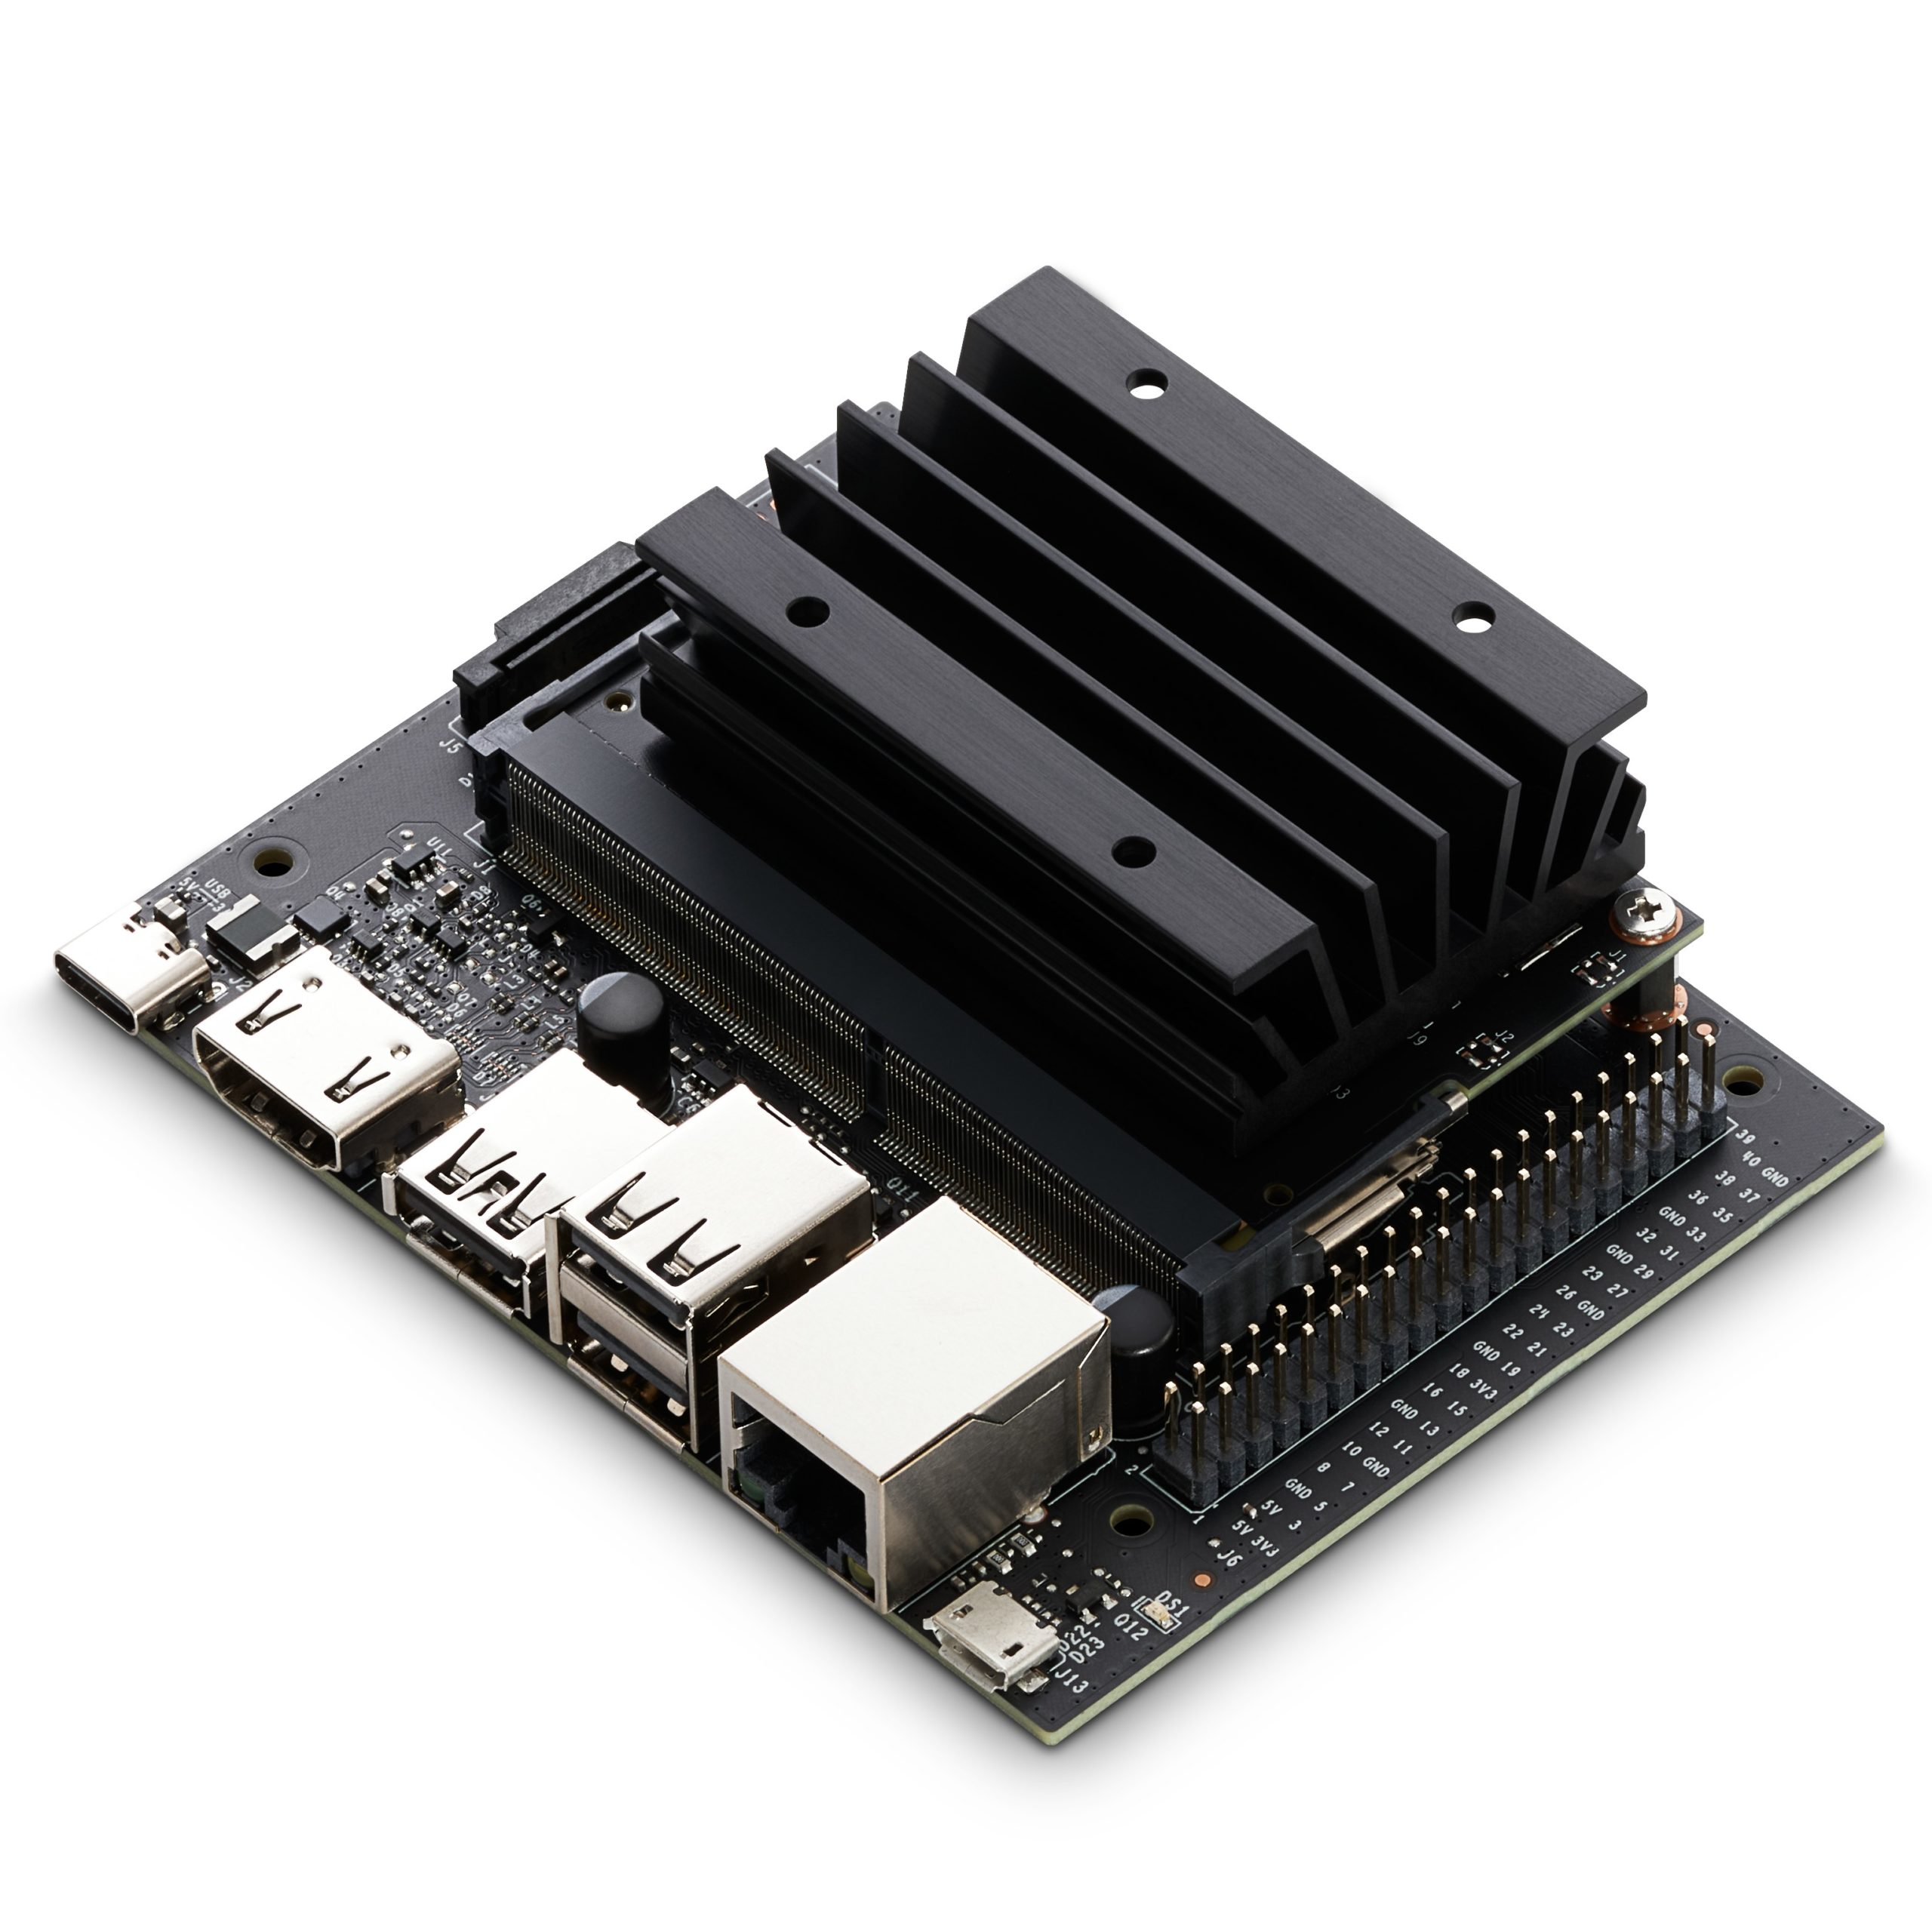
\includegraphics[width=0.5\textwidth]{jetson_nano.jpg}
	\caption{NVIDIA Jetson Nano}\label{fig:jetson-nano}
\end{figure}

\subsection{Cameras}

The selection of appropriate cameras is crucial for the effective operation of the parking management system. The primary requirements for these cameras include weather resistance to withstand heavy rain, the ability to transmit live video feeds to a central computer, and infrared detection capabilities for low-light conditions such as indoor garage parking or nighttime operations. Additionally, the cameras need to be capable of capturing high-quality images to facilitate accurate car detection and license plate identification.

To meet these requirements, several camera models were evaluated. Table \ref{tab:camera_comparison} presents a comparison of the considered options:

\begin{table}
	\begin{tabular}{|l|c|c|c|c|}
		\hline
		\textbf{Specification} & \textbf{Reolink RLC-811A} & \textbf{Lorex Fusion 2K} & \textbf{Eufy Cam S350} & \textbf{Arlo Ultra 2} \\
		\hline
		Resolution             & 4K (8MP)                  & 2K (4MP)                 & 4K (8MP)               & 4K (8MP)              \\
		\hline
		Waterproof             & IP66                      & IP66                     & Indoor only            & IP65                  \\
		\hline
		Infrared               & Yes                       & Yes                      & Yes                    & Yes                   \\
		\hline
		PoE                    & Yes                       & Yes                      & No                     & No                    \\
		\hline
		Price (\euro)          & 166                       & 300                      & 130                    & 399                   \\
		\hline
	\end{tabular}
	\caption{Comparison of Camera Options}\label{tab:camera_comparison}
\end{table}

After careful consideration, the Reolink RLC-811A, see \cref{fig:camera}, was selected as the optimal choice for this project. This camera offers 4K resolution, providing exceptional image clarity for accurate vehicle and license plate detection. Its IP66 weather resistance rating ensures durability in various outdoor conditions, including heavy rain. The camera's built-in infrared capabilities are sufficient for basic low-light operation and can be supplemented with additional infrared lighting when needed.

One of the key advantages of the Reolink RLC-811A is its support for Power over Ethernet (PoE). This feature allows for both power supply and data transmission through a single Ethernet cable, significantly simplifying installation and reducing wiring complexity. The camera's competitive price point of €166 also makes it an attractive option for large-scale deployments across multiple parking facilities.

While the Lorex Fusion 2K offers similar weather resistance and PoE capabilities, its lower 2K resolution may not provide the same level of detail required for accurate license plate recognition. However, it could be a viable alternative if budget constraints become more pressing, as it offers a good balance of features at a mid-range price point.

The Eufy Cam S350, despite its high 4K resolution and lower price, is not suitable for this project due to its lack of weather resistance and PoE capabilities. It is designed for indoor use only, which limits its application in outdoor parking environments.

The Arlo Ultra 2, while offering high-resolution 4K imaging and good weather resistance (IP65), lacks PoE support and comes at a significantly higher price point. Its wireless design, while potentially offering more flexible installation options, may not be ideal for a permanent, large-scale parking management system where consistent power and data connectivity are crucial.

\begin{figure}
	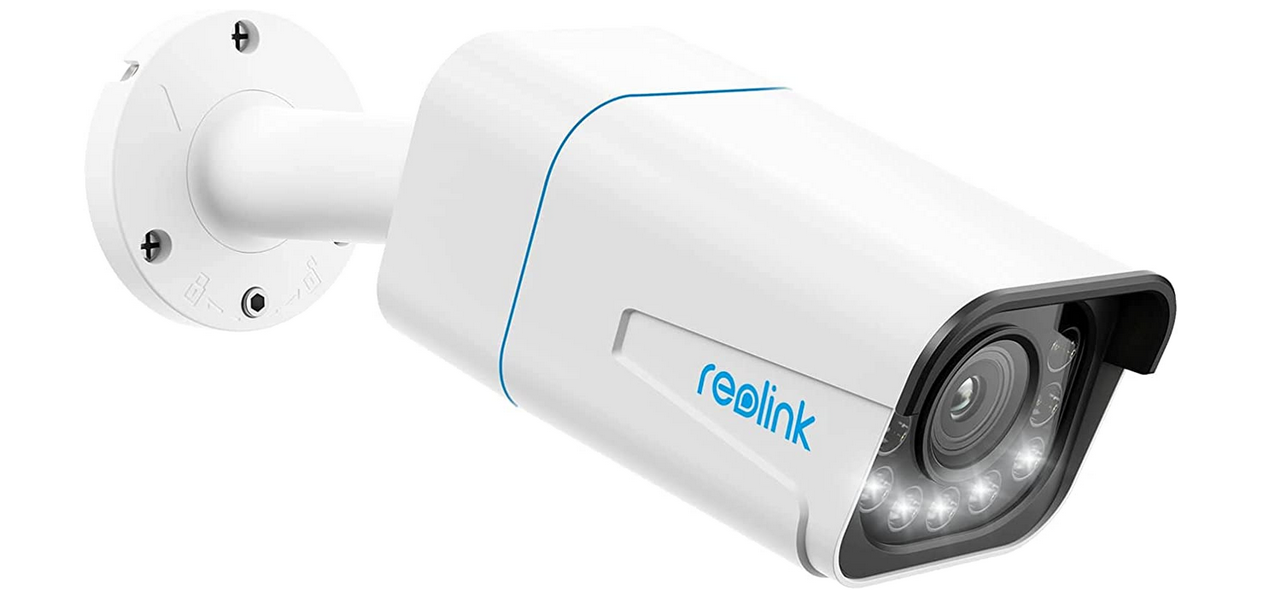
\includegraphics[width=0.5\textwidth]{camera.png}
	\caption{Reolink RLC-811A Camera}\label{fig:camera}
\end{figure}

\subsection{Internet Connectivity}

To provide connectivity from the on-board computer to the server, a networking connection needed to be established. As this deployment must be self-sufficient and not depend on the infrastructure of each community, a router with 4G connection is deployed. For this case, a simple 4G router was used, the TP-Link AC1200. This router offers 4G+ Cat6 connectivity and AC1200 wireless dual-band gigabit capabilities, making it suitable for providing reliable internet access for the parking management system. Moreover, this router has a built-in switch to be able to connect the cameras with the terminal.

\subsection{Server}

The server is the point of contact to connect users with the different communities, facilitating user authentication and enabling connections to specific community resources. It is built on a scalable architecture deployed in AWS (Amazon Web Services), chosen for its rapid time-to-market capabilities and inherent scalability.

AWS provides a cloud-based solution that allows the system to efficiently manage varying loads and adapt to user demand, which is essential for a parking management system that may experience fluctuating traffic patterns. This flexibility ensures that the system can scale up or down seamlessly, accommodating an increasing number of users and devices without compromising performance.

Moreover, AWS offers robust testing environments that allow developers to validate system functionalities before full deployment. This capability is crucial for ensuring reliability and performance under real-world conditions, as it enables iterative testing and refinement of the system components. By leveraging AWS's extensive infrastructure, the project can ensure high availability and resilience, minimizing downtime and enhancing user experience.

In summary, the choice of AWS not only supports the immediate needs of scalability and rapid deployment but also provides a solid foundation for ongoing testing and development, essential for maintaining an effective and responsive parking management solution.


